\section{Regelung und Handhabung von vorhandenen Informationen (ME)}
\todo[inline]{AW, ME: Zitate und Fußnoten anpassen}
In diesem Kapitel wird näher auf das Thema "'Wissensmanagement"' eingegangen. In einem weiteren Teil dieses Kapitels wird auf das Thema "'E-Learning"' näher Bezug genommen. Im letzten Punkt wird dargelegt, welche Sicherheitsaspekte an der Hochschule zum Einsatz kommen.

\subsection{Wissensmanagement}

Der Begriff "'Wissen"' nimmt eine wichtige Rolle im Wissensmanagement ein, denn "'Wissen"' entsteht durch die gedankliche Verarbeitung von Informationen im Gehirn (subjektives Gut). Es existieren verschiedene Wissensarten. Zum einen gibt es das "'explizite Wissen"' welches das Faktenwissen beinhaltet (aus Büchern, Datenbanken, Internet) und leicht zu erlernen ist und zum anderen wird nach "'impliziten Wissen"' unterschieden, welches schwerer zu erfassen ist, da es das Erfahrungswissen darstellt. Das Erfahrungswissen ist viel schwerer formulier- und kommunizierbar als das Faktenwissen. 

Nähere betrachtet ist Wissensmanagement die Organisation der Nutzung von Wissen für den Unternehmenserfolg. Doch gegenüber dem Informationsmanagement konzentriert sich der Ansatz des Wissensmanagement sehr stark auf den Menschen in seiner Funktion als Wissensträger. Häufig kommen IT-Systeme als Werkzeug des Wissensmanagements zum Einsatz, mit dem Ziel Wissenverluste zu kompensieren.\footnote{vgl. \url{http://wiki.infowiss.net/Wissensmanagement}, Abfragedatum: 19.06.2015}  Wissensmanagement ist eine Erweiterung der Informationsmanagementmaßnahmen. Dies bedeutet, dass nicht klar strukturierte Aufgaben, wie zum Beispiel Lernprozesse oder die Speicherung von Informationen besser bewältigt werden können.\footnote{vgl. \url{http://vfhinf.oncampus.de/loop/Abgrenzung_Informationsmanagement_und_Wissensmanagement}, Abfragedatum: 19.06.2015} 

Auch die Hochschule wird täglich mit dem Erwerb, der Entwicklung, dem Transfer sowie der Nutzung von Wissen konfrontiert. Für den Betrieb eines erfolgreichen Wissensmanagementsystems ist ein klares Regelwerk die Voraussetzung. 

Gilbert Probst erstellte 1999 ein theoretisches Modell der "'Kernprozesse des Wissensmangement"', um implizites Wissen besser in Unternehmen zu integrieren. Das Modell besitzt die Elemente Zielsetzung, Umsetzung und Bewertung. Im Modell wird zwischen einem "'äußeren Kreislauf"' (strategische Steuerungsaufgaben) und einem "'inneren Kreislauf"' (Umsetzung) unterschieden. Im inneren Kreislauf findet durch den äußeren Kreislauf eine Ergänzung der Elemente Zielsetzung (Wissensziele) und Messung (Wissensbewertung) statt. Die inneren Bausteine entsprechen den sechs Kernaktivitäten wie in Abbildung \ref{fig_wissensmanagament_probst} zu sehen ist. Somit bilden die acht Bausteine einen vernetzten Managementregelkreis. Zu sehen ist, dass die Kernaktivitäten untereinander in Verbindung stehen, jedoch nicht in vorgegebener Reihenfolge vollständig durchlaufen werden müssen. Dennoch muss darauf geachtet werden, dass alle Bausteine gleich berücksichtigt werden, da Probleme oft durch die Isolierung einzelner Kernaktivitäten entstehen.\footnote{vgl. \url{http://www.enzyklopaedie-der-wirtschaftsinformatik.de/wi-enzyklopaedie/lexikon/daten-wissen/Wissensmanagement/Wissensmanagement--Modelle-des/Wissensmanagement--Bausteinmodell-des-}, Abfragedatum: 19.06.2015.} 

\begin{figure}[h!]
	\centering
	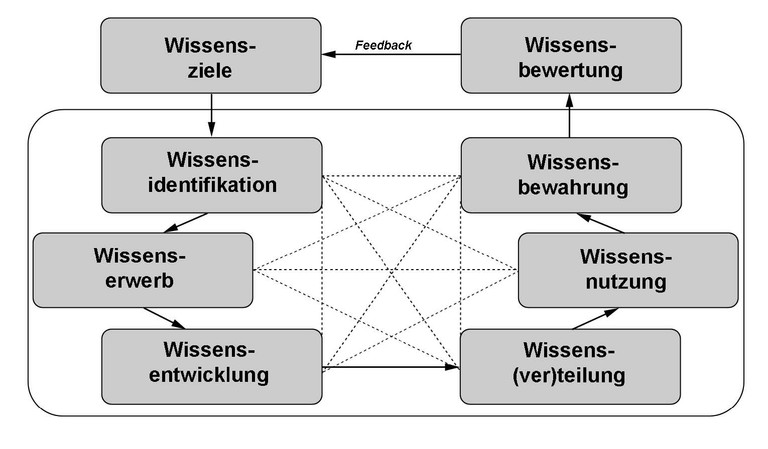
\includegraphics[width=8cm]{kapitel/gruppe2/bilder/wissensmanagament_probst}
	\caption{ Bausteinmodell des Wissensmanagement \protect\footnotemark}
	\label{fig_wissensmanagament_probst}
\end{figure}\footnotetext{\url {http://blog.protechnology.de/wp-content/uploads/2012/06/061812_1526_Wissensmana7.jpg}, Abfragedatum: 12.06.2015}

\subsection{E-Learning}
E-Learning ist das Lehren und Lernen, welches durch elektronische Medien unterstützt wird. Zum Einsatz kommen digitale Medien, wie zum Beispiel Computer oder Smartphones. Die Übermittlung von Lerninhalten erfolgt über verschiedenste Kanäle wie zum Beispiel das Internet, Computersoftware, Chatsysteme oder durch den Einsatz eines LMS (Learning Management System). Ein sehr bekanntes LMS ist die Plattform Moodle.\footnote{vgl. \url{http://team025.jimdo.com/unsere-vision/e-learning-eine-lernmethode-des-21-jahrhunderts/was-bedeutet-e-learning-eigentlich/}, Abfragedatum: 05.05.2015} In Kapitel \ref{subsubsection_e_learning_plattformen} wird darauf ebenfalls Bezug genommen.

\subsubsection{E-Learning an der Hochschule Emden/Leer}
E-Learning hat an der Hochschule einen hohen Stellenwert, da die Studiengänge Medieninformatik (Online) und seit 2015 Wirtschaftsinformatik (Online) akkreditiert  wurden. Nun soll dargelegt werden, ob in den Präsenzstudiengängen ebenfalls der E-Learning-Prozess Einzug gehalten hat.

\subsubsection{E-Learning in den Präsenzstudiengängen}
Es soll betrachtet werden, in welchen Präsenzstudiengängen E-Learning eingesetzt wird.

Der Fachbereich SAG (Soziale Arbeit und Gesundheit) ist der Vorreiter aller Fachbereiche mit der Einführung eines E-Learning Systems gewesen. SAG setzt mehr als 200 Onlinekurse im Präsenzstudium ein. Für die Anmeldung an verschiedenen Kursen sowie der Klausuranmeldung kommt ein Online-System zum Einsatz.

Es folgt dann der Fachbereich Technik, in dem E-Learning ebenfalls sehr stark verbreitet ist, da die Studiengänge Medieninformatik und Wirtschaftsinformatik als reine Onlinestudiengänge in diesem integriert sind.

Weniger stark wird E-Learning vom Fachbereich Wirtschaft betrieben. Das geringste Nutzungsverhalten ist im Fachbereich Seefahrt zu verzeichnen.

Trotz des unterschiedlichen Nutzungsverhaltens hat E-Learning in allen Fachbereich Einzug gehalten.

\subsubsection[Einsatz von E-Learning-Anwendungen]{Einsatz von E-Learning-Anwendungen in den Präsenzstudiengängen}
In diesem Abschnitt wird erläutert, ob die Anwendungen "'Adobe Connect"' und "'Moodle"' im Präsenzstudiengang eingesetzt werden.

\paragraph{Adobe Connect}\mbox{} \\

Adobe Connect ist eine Kommunikationsplattform zur Bereitstellung von Webmeeting- und E-Learning-Inhalten.

Ausschließlich der Fachbereich Technik (E+I) nutzt durch seine Onlinestudiengänge die Plattform Adobe Connect als Medium des visuellen Austausches von Bild und Sprache. In den Präsenzstudiengängen kommt die Plattform nicht zum Einsatz, da der persönliche Austausch von Studierenden und Dozenten in den täglichen Präsenzen stattfindet.

\paragraph{Moodle}\mbox{}\\\\
\label{paragraph_moodle}

Die Hochschule setzt als Lernplattform Moodle ein (siehe Abbildung \ref{fig_moodle}). Moodle ist ein freies objektorientiertes Kursmanagementsystem, welches den Fokus auf E-Learning Inhalte setzt.\footnote{\url{https://moodle.hs-emden-leer.de/moodle/}, Abfragedatum: 10.05.2015}

\begin{figure}[h!]
	\centering
	\includegraphics[width=8cm]{kapitel/gruppe2/bilder/moodle}
	\caption{Übersicht Moodle für alle \protect\footnotemark}
	\label{fig_moodle}
\end{figure}\footnotetext{\url {https://moodle.hs-emden-leer.de/moodle/}, Abfragedatum: 10.05.2015}

Durch den Einsatz von Moodle in allen Fachbereichen wird das volle Leistungsspektrum des Systems ausgenutzt. Folgende Funktionalitäten werden angeboten:

\begin{itemize}
	\item Lernvideos
	\item Vorlesungsskripte
	\item Forum
	\item Kalender
	\item Mail-Connect
\end{itemize}

Für jeden Fachbereich wird der volle Funktionsumfang der Plattform zur Verfügung gestellt, auch wenn nicht jeder Fachbereich jeden Service nutzt. 

\subsubsection{Zentrale Informationsbereitstellung durch Datenlaufwerke}
\label{zentrale_Datenlaufwerke}
Für alle Beteiligten der Hochschule werden drei Datenlaufwerke (siehe Abbildung \ref{fig_zugriff_datenlaufwerke_extern}) auf den Fileservern des eigenen Rechenzentrums zur Verfügung gestellt.\footnote{\url{https://connect.hs-emden-leer.de/cgi-bin/welcome}, Abfragedatum: 10.05.2015}

\begin{figure}[h!]
	\centering
	\includegraphics[width=8cm]{kapitel/gruppe2/bilder/zugriff_auf_laufwerke_extern}
	\caption{Zugriff auf die Datenlaufwerke von extern \protect\footnotemark}
	\label{fig_zugriff_datenlaufwerke_extern}
\end{figure}\footnotetext{\url {https://connect.hs-emden-leer.de/cgi-bin/portal}, Abfragedatum: 10.05.2015}


\paragraph{Laufwerk Z}\mbox{} \\

Auf dem "'Laufwerk Z"' befinden sich die Daten des Home-Verzeichnisses jedes einzelnen Benutzers. Meldet sich dieser an beliebigen Rechnern des internen Rechnerpools an, werden die Inhalte seins Home-Verzeichnisses automatisch eingebunden. Der interne Zugriff auf die eigenen Dateien ist von jedem Rechner des Pools möglich, da servergespeicherte Profile zum Einsatz kommen. Auch von extern können die Studierenden problemlos auf die Ressourcen der Datenlaufwerke zugreifen.

\paragraph{Laufwerk Y}\mbox{} \\

Für den gemeinsamen Austausch der Daten wurde das "'Laufwerk Y"' eingerichtet. Hier werden zentral Ressourcen für alle Studierenden und Lehrenden aus Emden zum Austausch zur Verfügung gestellt.

\paragraph{Verzeichnis Lehrende aus Leer}\mbox{} \\

Zusätzlich zum Transferlaufwerk wird das Laufwerk "'Verzeichnis Lehrende aus Leer"' zur Verfügung gestellt. Dieses Laufwerk wird zur Bereitstellung von Inhalten (Vorlesungsmaterialien, Skripte, Übungen) verwendet.

\subsubsection{Moodle vs. Datenlaufwerke für Präsenzstudenten}
An der Moodle-Lernplattform melden sich die Nutzer über eine webbasierte Oberfläche am System an. Um Dateien zur Verfügung zu stellen, muss auf der Weboberfläche zu den gewünschten Reitern navigiert werden.

Stellt man die Datenlaufwerke (Laufwerk Y und das Transferlaufwerk "Verzeichnis Lehrende aus Leer") der Moodle-Plattform gegenüber und betrachtet nur den Aspekt des Datenaustausches, so wird deutlich, dass der Dateiaustausch über Datenlaufwerke in Bezug auf Komfort und Aufwand deutlich besser für die Präsenzstudierenden geeignet ist, als die Dateiablage über die Moodle-Plattform. Die über die Datenlaufwerke zur Verfügung gestellten Inhalte können von den Studierenden mit wenig Aufwand intuitiv erreicht werden.

Aus dem Interview mit Günter Müller kristallisierte sich heraus, dass der Fachbereich Wirtschaft die Datenlaufwerke am stärksten und der Fachbereich Technik und andere Fachbereiche diese weniger stark nutzen.

\subsection{Sicherheitsaspekte}
In diesem Kapitel wird auf die bereits verwendeten Sicherheitsrichtlinien an der Hochschule detaillierter eingegangen. Weiterhin wird geprüft, ob ein IT-Service-Management-Prozess  umgesetzt ist.

\subsubsection{Sicherheitsrichtlinien an der Hochschule}
Der Einsatz von Sicherheitsrichtlinien ist ein wichtiges Thema an Hochschulen. Sicherheitsrichtlinien beschreiben die Sicherstellung von Verfügbarkeit, Integrität, Vertraulichkeit und Authentizität von Informationen.\footnote{vgl. \url{http://www.datenschutz-berlin.de/content/technik/begriffsbestimmungen/verfuegbarkeit-integritaet-vertraulichkeit-authentizitaet}, Abfragedatum: 11.05.2015}

An der Hochschule werden, als Basis für die Informationssicherheit Teile des IT-Grundschutz-Kataloges umgesetzt. Nicht alle Empfehlungen des BSI (Bundesamt für Sicherheit in der Informationstechnik) sind an einer kleinen Hochschule, wie die Hochschule Emden/Leer es ist,  umsetzbar. Das BSI ist eine nationale Sicherheitsbehörde deren Ziel es ist, die IT-Sicherheit in Deutschland voran zu bringen. Somit ist das BSI ein zentraler IT-Sicherheitsdienstleister des Bundes.\footnote{vgl. \url{https://www.bsi.bund.de/DE/DasBSI/dasbsi_node.html}, Abfragedatum: 11.05.2015}

An den Serverräumen der Hochschule ist die Umsetzung der IT-Grundschutzmaßnahmen deutlich zu erkennen.
Folgende physikalische Schutzmaßnahmen wurden in den Serverräumen umgesetzt:

\begin{itemize}
	\item einbruchssicher
	\item feuergemeldet
	\item videoüberwacht
	\item Lage der Serverräume im 1. OG (Wasserschutz)
\end{itemize}

\subsubsection{Einsatz von ITIL}
Die IT Infrastructure Libary (ITIL) ist eine Sammlung von Best Practises zur Umsetzung eines IT-Service-Management-Prozesses (siehe Kapitel \ref{itil}). In diesem Regelwerk werden die für den Betrieb einer IT-Infrastruktur notwendigen Prozesse und Werkzeuge beschrieben.\footnote{vgl. \url{http://www.dxperts.de/wordpress/dienstleistungen/it-infrastructure-library-itil}, Abfragedatum: 10.05.2015} ITIL gilt als De-Facto-Standard. Eine Zertifizierung ist nicht für Unternehmen, sondern nur für Personen möglich. Unternehmen können sich nach ISO 20000 zertifizieren lassen.\footnote{vgl. \url{http://wirtschaftslexikon.gabler.de/Definition/itil.html}, Abfragedatum: 10.05.2015}

Der ITIL-Prozess ist an der Hochschule nicht umgesetzt, da die Personaldecke für die Umsetzung eines 1st- und 2nd-Level Supports nicht gegeben ist.

\subsubsection{Umsetzung von ISO/IEC 27001}
Die ISO/IEC 27001 Zertifizierung wird auf Basis des IT-Grundschutzes vergeben. Durch die Zertifizierung des ISO/IEC 27001 Standards haben Unternehmen, Behörden und Organisationen die Möglichkeit, ihre Bemühungen um Informationssicherheit nach innen und außen zu dokumentieren.\footnote{vgl. \url{https://www.bsi.bund.de/DE/Themen/ZertifizierungundAnerkennung/Zertifizierung27001/GS_Zertifizierung_node.html}, Abfragedatum: 10.05.2015}

Das Einsatzszenario ist an der Hochschule nicht gegeben, da für Umsetzung die Personaldichte zu gering ist. Für die Erfüllung der Zertifizierung würde ein riesiger Personaloverhead entstehen.

\subsubsection{Fazit Sicherheitsrichtlinien}
Abschließend ist zu sagen, dass an der Hochschule der IT-Sicherheitsaspekt eine sehr entscheidende Rolle spielt. Als kleine Hochschule ist es auf Grund der Personaldichte nicht möglich, alle Empfehlungen des BSI-Grundschutzes, ITIL und ISO/IEC 27001 umzusetzen. Jedoch sucht sich die Hochschule aus den Regelwerken die Empfehlungen heraus, die auf Grund der Personaldichte umsetzbar sind. Dies bildet eine sehr gute Basis im Hinblick auf das sehr anspruchsvolle Thema IT-Sicherheit.
